\subsection{Introducción}

La etapa de entrada de un amplificador cumple con la función de restar a la entrada la señal proveniente de la realimentación, para así obtener la señal deseada de error, a partir de la cual se confecciona la salida del sistema. Para este análisis se trabajó con la información obtenida a partir del libro ``Audio Power Amplifier Design Handbook'' de Douglas Self, $5^{ta}$ edición.
%\footnote{D. Self, Audio Power Amplifier Design Handbook, 5ta ed. Kidlington: Elsevier Science, 2014.}

\subsection{Distorsión}

La distorsión puede ser provocada o provenir de distintas fuentes. Los amplificadores que se valen del uso de pares diferenciales como entrada se caracterizan por poseer un bajo offset de continua, dado a la cancelación de los voltages de $V_{BE}$. Pero mucho más notorio e importante es que la corriente de mantenimiento no atraviesa la red de realimentación. Finalmente, una ventaja también a destacar es que posee una linealidad superior a las entradas basadas en un solo transistor. Se puede observar la comparación de distorsión entre una etapa diferencial frente a una individual en la Figura (\ref{fig:thd1}).

Es muy importante reflejar que esta etapa debe la que posee la mínima distorsión, por sobre las demás, ya que las señales que maneja son pequeñas, dándose el aumento de estas en la etapa de amplificación.    
\begin{figure}[H]
\centering
	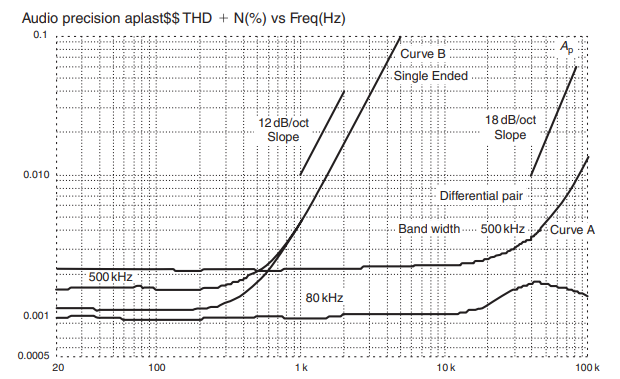
\includegraphics[width=0.6\textwidth]{ImagenesInput-Stage/thd1.PNG}
	\caption{Comparación de THD en función de la frecuencia.}
	\label{fig:thd1}
\end{figure}

Si bien, seleccionando adecuadamente las resistencias del circuito se puede balancear el par, quedan pendientes ciertos parámetros. Las corrientes de colectores deben ser lo más similares posibles. Debe existir una precisión del $1\%$ o mejor para poder optimizar la linealidad del la etapa, y de esta forma, reducir la distorsión en altas frecuencias.
\begin{figure}[H]
\centering
	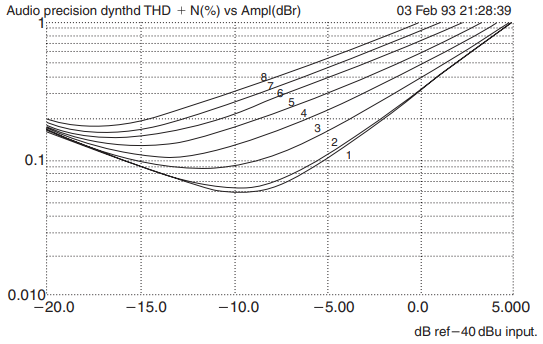
\includegraphics[width=0.6\textwidth]{ImagenesInput-Stage/thd2.PNG}
	\caption{THD en función de la entrada (en $dBu$, nivel de referencia $0.7746 \ V$) al variar el balance de la corriente del colector . Número de curva y distorsión especificadas en la Tabla (\ref{tab:thd2}).}
	\label{fig:thd2}
\end{figure}

\begin{table}[H]
\centering
\begin{tabular}{cc}
\hline
\textbf{Número de curva} & \textbf{Variación $\mathbf{I_C}$ [\%]} \\ \hline
1                        & 0                    \\
2                        & 0.5                  \\
3                        & 2.2                  \\
4                        & 3.6                  \\
5                        & 5.4                  \\
6                        & 6.9                  \\
7                        & 8.5                  \\
8                        & 10             		\\
\hline
\end{tabular}
\caption{Número de curva y distorsión de la Figura (\ref{fig:thd2}).}
\label{tab:thd2}
\end{table}

Una opción valida (e implementada en este diseño) se basa en el uso de una fuente de corriente compensada para polarizar el par. Además, se emplean resistencias en los emisores para ajustar dicho parámetro. Es importante recordar que dichos elementos no deben ser lo suficientemente grandes como para que afecte el ruido térmico.  

\subsection{Linealidad y corriente de colector}

La transconductancia aumenta con la corriente de colector. Elevar este último parámetro es posible y relativamente sencillo. Una técnica empleada para poder mejorar la linealidad en altas frecuencias consiste en aumentar la corriente mencionada para luego reducirla a través del lazo de realimentación negativa. Esta no linealidad es atribuida a la resistencia del $R_E$ del emisor, la cual no es una resistencia física, sino que una resultante de la expresión de la pendiente de la corriente de colector. 

La corriente de mantenimiento a la entrada es uno de los parámetros que define el máximo slew rate (SR). Otro factor importante que lo limita es el polo dominante proveniente del capacitor de Miller. Este último es solucionado por los requerimientos que se deben cumplir para conseguir la estabilidad. Por otro lado, aumentar la corriente de colector puede aumentar el factor de SR sin afectar la estabilidad, siempre y cuando, la transconductancia se mantenga en el valor deseado. 

A pesar de ello, existen límites para esta corriente. El aumento de las corrientes de bias, como la caída de tensión a través de las resistencias son algunos ejemplos. El factor más limitante es la potencia disipada a lo largo de esta etapa, ya que no siempre deja margen para incrementar la $I_C$. 

\subsection{Ruido}
El ruido existente en la etapa de entrada surge de los componentes activos y las resistencias que se presentan en la entrada. Las condiciones de operación de los transistores se encuentran limitadas por los factores de SR y linealidad. Por otro lado, ya que el ruido es una función que dependen de $I_C$, bastan con ajustar dicho parámetro para poder reducir el ruido. 

Además de reducir las resistencias existentes en la etapa de entrada para así reducir el ruido térmico existente, es posible realizar el mismo efecto haciendo lo mismo con la resistencia observada a la salida del lazo de realimentación negativa. Este último paso es más delicado ya que puede generar grandes cambios en el sistema.

\subsection{Limitación en banda}
Se sabe que  existen etapas que acumulan cambios de la fase, siendo estas las altas frecuencias, las cuales tienden a ser más inestables y generar oscilaciones. Es así que se puede llegar a dañar los dispositivos a la salida del sistema por sobrecalentamiento, entre otros motivos. Esto es causado por la distorsión del amplificador y el incremento de la ganancia de lazo abierto. Limitar en banda esta ganancia evita que la señal del realimentador.

\subsection{Calculo de componentes}
La disposición establecida para la etapa de entrada es la siguiente:
\begin{figure}[H]
\centering
	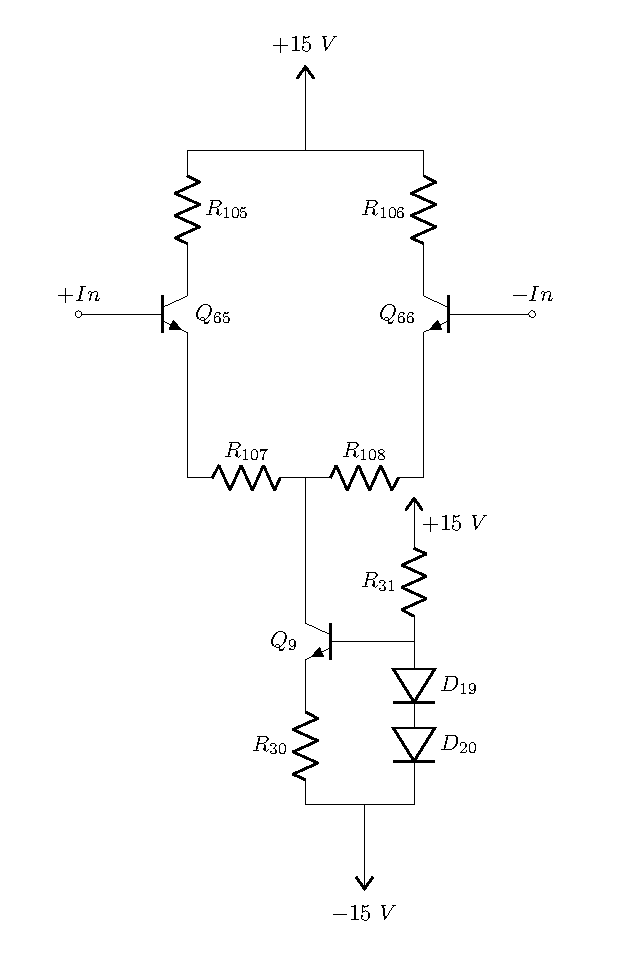
\includegraphics[width=0.5\textwidth, page=1]{ImagenesInput-Stage/Input.pdf}
	\caption{Etapa de entrada.}
	\label{fig:input}
\end{figure}

Para poder seleccionar los elementos y parámetros que componen la etapa de entrada, ya que se polariza ambos transistores por una fuente de corriente compensada, se comenzó por dicha fuente, para así obtener la siguiente ecuación:
\begin{equation}
	-15 \ V - 2V_{D} + V_{BE} + 15 \ V = I_O R_{30} 
\end{equation}

Recorriendo la malla de entrada:
\begin{equation}
	- V_{BE} - \frac{R_V}{2} I_C - R_{30} I_O - V_{CEQ9} + 15 \ V = 0
\end{equation}

Recorriendo la malla del par, se llega a la expresión:
\begin{equation}
	15 \ V - R_{105} I_C - V_{CEQ65} - \frac{R_V}{2} I_C - R_{30} I_O - V_{CEQ9} + 15 \ V = 0
\end{equation}

Además, se coloca un preset en los emisores del par para poder ajustar la corriente que circula, en caso de ser necesario. Dado esto último, la ganancia del par diferencial con el preset viene dada por la expresión:
\begin{equation}
	\Delta V_D = \frac{h_{fe} R_D}{2 h_{ie} + h_{fe} R_V} = \frac{R_{105}}{2 \frac{V_T}{I_C} + R_V}
\end{equation}
siendo $I_C = \frac{I_O}{2}$, $V_T \approx 25 \ mV$ y $R_V = R_{107} + R_{108} = 2 R_{107} $.

Se selecciona $R_V = 1 \ k\Omega$ ya que este es un valor típico para las resistencias con esta funcionalidad. Se busca que la ganancia de esta etapa sea baja, que no altere mucho la señal (no mayor a $10$ veces) y que los transistores se encuentren bien polarizados. Mediante el uso de las ecuaciones previamente mencionadas, se obtienen los siguientes valores de interés:
\begin{itemize}
	\item Para la fuente de corriente: $I_O = -9.41 \ mA$ y $R_{30} = 68 \ \Omega$.
	\item Para la resistencia del colector: $R_{105} = 2 \ k\Omega$.
\end{itemize}